\subsection{Der Data-Lake-Prototyp}
Ein Data Lake basiert darauf, dass zuerst alle Daten in ihrem Rohformat gespeichert werden.
Dadruch fällt der Aufwand einer Transformation bei der Integration von neuen Daten weg.
Gleichzeitig bleiben auch alle Informationen bleiben für Analysen erhalten\parencite{datalake_03}.
Neben dem Speichern und Bereitstellen von Daten ist eine weitere Aufgabe eines Data-Lake-Systems die verwaltung von Metadaten.


Wärend dem Masterprojekt \citetitle{prototyp} \parencite{prototyp} an der Hochschule Niederrhein wurde bereits eine Data-Lake-System-Prototyp entwickelt.
In \fref{fig:prototyp-architektur} ist ein Überblick über dessen Architektur zu sehen.
Es handelt sich hierbei um eine Client-Server-Anwendung.
Der Client besteht aus einer Web-Anwendung über die Benutzer mit dem Data-Lake-System interagieren.
Er kommuniziert mit dem Server über eine REST-API, die auch durch andere Clients verwendet werden könnte.
Die Datenverarbeitung wird über ein Apache Spark Cluster gelöst.
Zum Speichern der Daten stehen drei verschieden System zu verfügung.
Eine Postgres Datenbank für strukturierte, eine MongoDB für semistrukturierte und ein HDFS für unstrukturierte Daten.

\begin{figure}
    \centering
    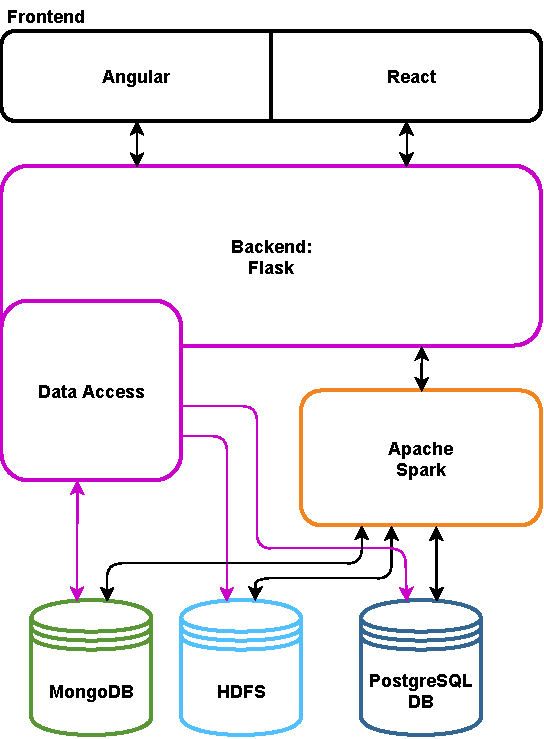
\includegraphics{Grafiken/data_lake_prototype_arch.pdf}
    \caption{Architektur des Prototypen, \citetitle[Quelle:][S. 2]{prototyp}}
    \label{fig:prototyp-architektur}
\end{figure}

Die Verarbeitung der Ingestion ist im Prototyp Abhängig von der Datenquelle und dem ausgewählten Zielspeicher.
In \fref{fig:prototyp-ingestion} sind die verschiedenen Wege zu sehen.
Diese Verarbeitungsweise hat zwei Probleme, die in der neuen Ingestion gelöst werden müssen.
Dadurch, dass der Benutzer aus den verschiedenen Speichern ein Ziel auswählt, können hier leicht Probleme entstehen, falls die Datenquelle nicht mit dem Format des Speichers kompatibel ist.
Außerdem sind die Verarbeitungsweisen der Quellen zu den Speichern fest im Code des Servers festgehalten.
So ist es nicht möglich wärend der Laufzeit neue Datenquellen zu integrieren.

\begin{figure}
    \centering
    \subfigure[Datenbank-Ingestion]{
        \label{fig:prototyp-db-ingeston}
        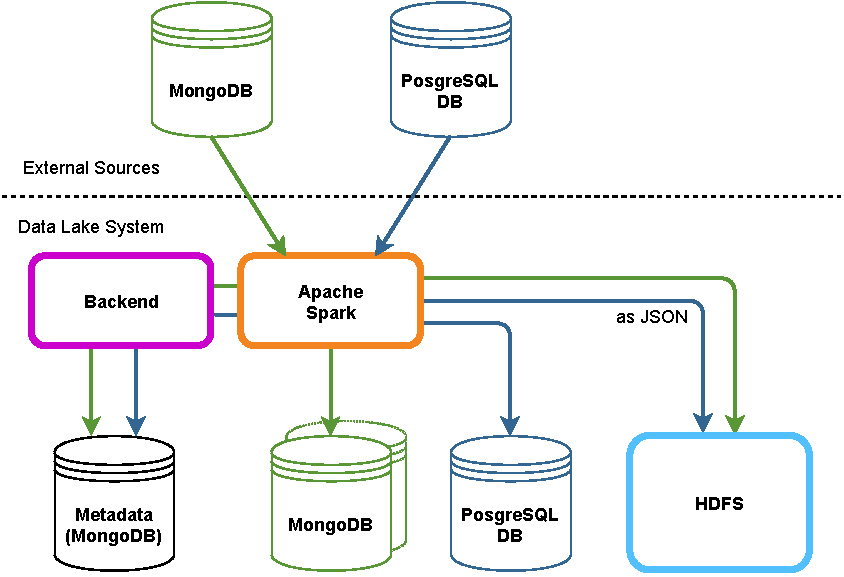
\includegraphics[width=.45\textwidth]{Grafiken/db_ingestion.pdf}
    }
    \subfigure[Datei-Ingestion]{
        \label{fig:prototyp-file-ingeston}
        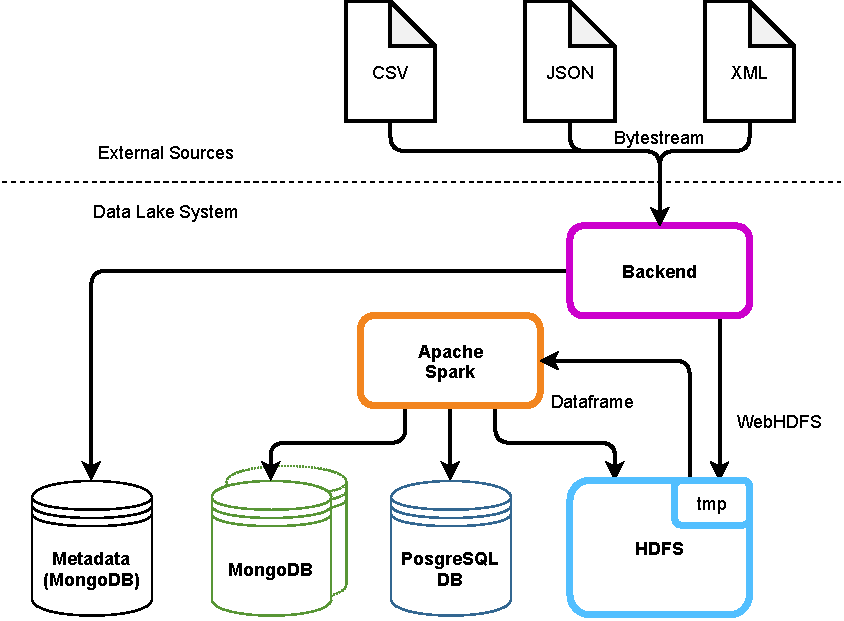
\includegraphics[width=.45\textwidth]{Grafiken/file_ingestion.pdf}
    }
    \caption{Ingestion-Verarbeitung des Prototypen, \citetitle[Quelle:][S. 3]{prototyp}}
    \label{fig:prototyp-ingestion}
\end{figure}